\chapter{Graphüberdeckung}

Wie zuvor gesehen, existieren verschiedene Coverage-Kriterien um Testabdeckung zu prüfen.
Graphcoverage ist hierbei eine Herangehensweise um graphenbasierte Datenstrukturen zu überdecken.
Graphen können nämlich ähnliche Probleme aufweisen wie vorheriges Beispiel der Addition.
Die Addition zweier 64-bit Integer ist wenigstens endlich, Graphenstrukturen haben sogar unter Umständen unendliche Testräume.
Umso wichtiger ist es hier, dass Überdeckungskriterien formuliert werden können, die diesen möglicherweise unendlichen Suchraum
stark verkleinern und dennoch eine ausreichende Testung ermöglichen.
Da wir vorher ergründet haben, dass GraphQL sich als gerichteten Graph darstellen lässt, können wir nun die Graphcoverage nutzen, um Tests mithilfe der Grapcoverage zu erstellen.
Wie genau die Coverage erstellt wird und daraus Tests resultieren, werden im folgenden geklärt.
Gerichtete Graphen sind die Grundlage für viele Coverage-kriterien, wobei die Grundidee hierbei ist,
Sachverhalte als Graphen zu modellieren und dann eine ausreichende Überdeckung zu finden. \cite[vgl. Software-testing S. 27 2.1]{software-testing}
In $4.1.2$ wurden gerichtete Graphen bereits eingeführt, daher können wir direkt fortfahren und verschiedene
Kriterien definieren, die einen Graphen überdecken.
Wir erklären zuerst verschiedene Techniken, die einen Graphen überdecken und erklären dann ihre Anwendung
an Beispielen.
Erst sortieren wir Graphcoverage ein im Kontext von Code-Coverage und bilden im zweiten Schritt eine Coverage für GraphQL\@.

\section{Graphüberdeckung allgemein}

Um Graphcoverage zu nutzen, verfeinern wir zuerst die allgemeine Definition von gerichteten Graphen.
Ein gerichteter Graph ist ein Paar $G = (V, E)$ zweier disjunkter Mengen mit $E \subseteq V^2$ wobei alle Elemente aus E gerichtete Kanten sind. [vgl. 4.1.2]
Die Definition erweitern wir nun mit:

\begin{description}
    \item[Menge N] von Knoten
    \item[Menge N_{0}] von Anfangsknoten, wobei N_{0} $\subseteq$ N
    \item[Menge N_{f}] von Endknoten, wobei N_{f} $\subseteq$ N
    \item[Menge E] von Kanten, wobei E $\subseteq$ N x N. Hierbei ist die Menge als init{x} x target{y} definiert.
\end{description}~\cite[2.1 Overview]{software-testing}

Mithilfe dieser Definition können nun zum Beispiel Kontrollflussgraphen abgebildet werden indem die Einstiegspunkte die Anfangsknoten sind und die Endknoten die Austrittspunkte.
Ein Pfad innerhalb von eben definierten Graphen, mit möglicher Länge Null, der in einem Knoten $N_{0}$ startet und in einem Knoten $N_{f}$ endet, nennt sich Testpfad \cite[vgl. S. 28]{software-testing}
Ziel ist es nun mit hilfe von Coverage-Kriterien Testpfade zu ermitteln die unser Problem ausreichend testen - was hierbei ausreichend ist, ist von Fall zu Fall unterschiedlich.

\section{Graphüberdeckung Kriterien}

Mithilfe voriger Definition können wir nun Coveragekriterien entwickeln, die uns Testpfade liefern, die je nach Kriterium für eine spezielle Abdeckung
des Graphens mit Test-Requirements sorgen.

\subsection{Node Coverage}

Node-Coverage ist ein Coveragekriterium, dass alle Knoten, die von $N_{0}$ erreichbar sind, in einem Graphen abdecken soll.
Definieren wir folgenden, sehr einfachen Graphen:

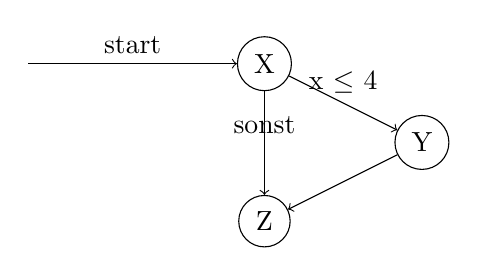
\begin{tikzpicture}
    \node[circle, draw] (n1) at (2,2) {X};
    \node[circle, draw] (n2) at (4,1) {Y};
    \node[circle, draw] (n3) at (2,0) {Z};

    \draw[->] (-1,2) -- node[above] {start} (n1);
    \draw[->] (n1) -- node[above] {x $\le$ 4} (n2);
    \draw[->] (n2) -- (n3);
    \draw[->] (n1) -- node[above] {sonst} (n3);
\end{tikzpicture}

So wäre die Node-Coverage mit einem Test einzigen Test erfüllbar.
Dieser ist der Pfad $X \rightarrow Y \rightarrow Z$.
Es ist auch denkbar, dass wir zwei Pfade oder mehr nutzen allerdings erfüllt dieser Pfad schon unser Kriterium daher geben wir uns vorerst zufrieden.
Wir sehen schnell, dass dieser Ansatz noch Lücken aufweist, da der Pfad $X \rightarrow Y \rightarrow Z$ das Kriterium erfüllt, allerdings wird eine Kante $X \rightarrow Z$ nicht im
Test berücksichtigt und kann somit ungetestet bleiben.
Wir führen also noch andere Kriterien ein, die eher geeignet wären.

\subsection{Edge-Coverage}

Edge-Coverage ist ein Coveragekriterium, dass die Kanten in einem Graphen abdecken soll.
Ziel der Edge-Coverage ist es, dass jede Kante des Graphens durch mindestens einen Test abgedeckt wird.
Um die Edge-Coverage für vorheriges Beispiel zu erreichen, benötigen wir schon zwei Routen.
Der Graph:

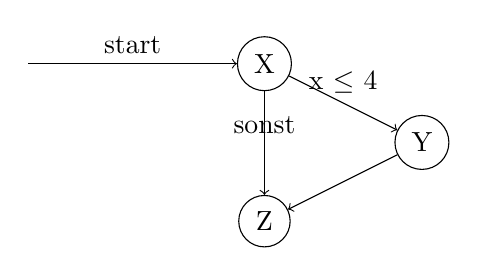
\begin{tikzpicture}
    \node[circle, draw] (n1) at (2,2) {X};
    \node[circle, draw] (n2) at (4,1) {Y};
    \node[circle, draw] (n3) at (2,0) {Z};

    \draw[->] (-1,2) -- node[above] {start} (n1);
    \draw[->] (n1) -- node[above] {x $\le$ 4} (n2);
    \draw[->] (n2) -- (n3);
    \draw[->] (n1) -- node[above] {sonst} (n3);
\end{tikzpicture}

wird über die Pfade $X \rightarrow Y \rightarrow Z$ und $X \rightarrow Z$ überdeckt.
Edge-Coverage hat allerdings auch Probleme Graphen vollständig zu überdecken.
Man nehme folgendes Beispiel:

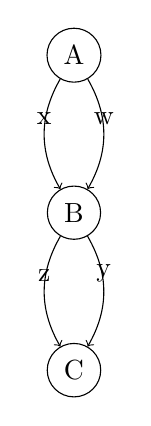
\begin{tikzpicture}
    \node[circle, draw] (a) at (4,4) {A};
    \node[circle, draw] (b) at (4,2) {B};
    \node[circle, draw] (c) at (4,0) {C};

    \draw[->, bend left=30] (a) to node[above] { w } (b);
    \draw[->, bend right=30] (a) to node[above] { x } (b);
    \draw[->, bend left=30] (b) to node[above] { y } (c);
    \draw[->, bend right=30] (b) to node[above] { z } (c);
\end{tikzpicture}

Pfade die laut Edge-Coverage ausreichen um den Graphen zu überdecken wären: \\
$ x \rightarrow z $ \\
$ w \rightarrow y $ \\
Hierbei wird allerdings außer acht gelassen, dass in $x$ auch Änderungen passieren können die Auswirkungen im Programm haben können.
So sind die Routen $ x \rightarrow y $ und $ w \rightarrow z $ in der Edge-Coverage nicht berücksichtigt.
Allerdings wären diese auch zu testen.
Wir sehen also, dass wir immer noch kein ideales Kriterium gefunden haben.


\subsection{Edge-Pair Coverage}

Das Edge-Pair Coveragekriterium ist eine Erweiterung der Edge-Coverage, indem hier auch die Beziehungen von einzelnen Kanten untereinander berücksichtigt werden um das zuvor
aufgetretene Problem zu lösen.
Nach \cite[Introduction to Software Testing]{software-testing} ist Edge-Pair Coverage: ''Alle erreichbaren Pfade von Länge bis zu 2 im Testgraphen''.
Ziel dieses Coverage-Kriteriums ist es, dass alle möglichen Kantenpaare abgedeckt sind.
Eben definiertes Beispiel hätte mit Edge-Pair Coverage eine Überdeckung mit: \\
$ x \rightarrow z $ \\
$ w \rightarrow y $ \\
$ x \rightarrow y $ \\
$ w \rightarrow z $

Dieses simple Beispiel wird durch Edge-Pair Coverage gut abgedeckt.
Edge-Pair Coverage neigt allerdings dazu, extrem große Suchräume zu erzeugen und nur Pfadkombinationen bestimmter Länge zu betrachten. \cite[vgl. S. 35]{software-testing}
Hierdurch werden bestimmte Kombinationen von Pfaden immer noch nicht berücksichtigt.

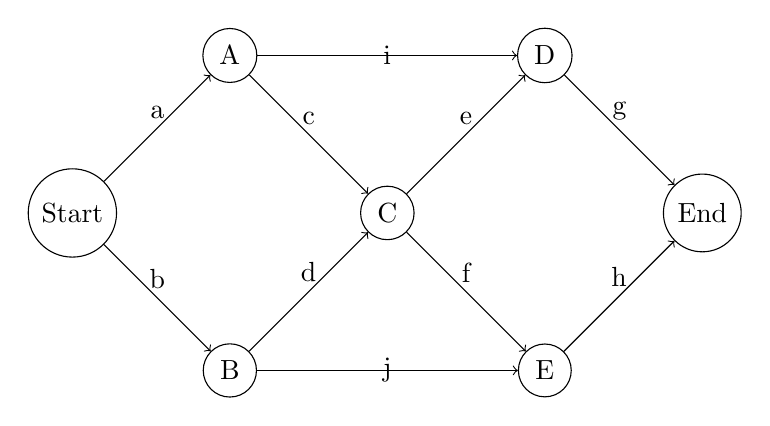
\begin{tikzpicture}
    \node[circle, draw] (start) at (0,0) {Start};
    \node[circle, draw] (a) at (2,2) {A};
    \node[circle, draw] (b) at (2,-2) {B};
    \node[circle, draw] (c) at (4,0) {C};
    \node[circle, draw] (d) at (6,2) {D};
    \node[circle, draw] (e) at (6,-2) {E};
    \node[circle, draw] (end) at (8,0) {End};

    \draw[->] (start) to node[above] { a } (a);
    \draw[->] (start) to node[above] { b } (b);
    \draw[->] (a) to node[above] { c } (c);
    \draw[->] (b) to node[above] { d } (c);
    \draw[->] (c) to node[above] { e } (d);
    \draw[->] (c) to node[above] { f } (e);
    \draw[->] (d) to node[above] { g } (end);
    \draw[->] (e) to node[above] { h } (end);
    \draw[->] (a) to node[out=30, in=150] { i } (d);
    \draw[->] (b) to node[out=-30, in=210] { j } (e);
\end{tikzpicture}

Nach der Definition von Edge-Pair Coverage ermitteln wir erstmal alle Pfadkombinationen der Länge ''bis zu 2''
Dies wären:

$Start \rightarrow A \rightarrow C$ \\
$Start \rightarrow A \rightarrow D$ \\
$Start \rightarrow B \rightarrow C$ \\
$Start \rightarrow B \rightarrow E$ \\
$A \rightarrow C \rightarrow D$ \\
$A \rightarrow C \rightarrow E$ \\
$B \rightarrow C \rightarrow D$ \\
$B \rightarrow C \rightarrow E$ \\
$A \rightarrow D \rightarrow End$ \\
$B \rightarrow E \rightarrow End$ \\
$C \rightarrow D \rightarrow End$ \\
$C \rightarrow E \rightarrow End$ \\

Hierdurch ergeben sich dann diese Testpfade:

$Start \rightarrow  A \rightarrow  C \rightarrow  D \rightarrow  End$ \\
$Start \rightarrow  A \rightarrow  C \rightarrow  E \rightarrow  End$ \\
$Start \rightarrow  B \rightarrow  C \rightarrow  D \rightarrow  End$ \\
$Start \rightarrow  B \rightarrow  C \rightarrow  E \rightarrow  End$ \\

allerdings fehlen auch hier wieder Pfade. \\
Zum Beispiel der Pfad $Start \rightarrow A \rightarrow D \rightarrow End$ fehlt.
Hierdurch bleiben wieder Teile des Graphens unüberdeckt.

\subsection{Prime-Path Coverage}

Die Prime-Path Coverage verlangt, dass jeder (Prime)Primärpfad durch mindestens einen Testpfad abgedeckt sein muss.
Ein Primärpfad ist definiert als ein einfacher Pfad, der nicht vollständig als zusammenhängender Teil in einem anderen einfachen Pfad enthalten ist. \cite[vgl. S. 35]{software-testing}
Hierbei ist ein einfacher Pfad dann  ein Pfad, in dem keine Kanten und keine Knoten wiederholt werden,
mit Ausnahme möglicherweise des ersten und letzten Knotens (wenn sie gleich sind, handelt es sich um einen Kreis).
In diesem Graphen:

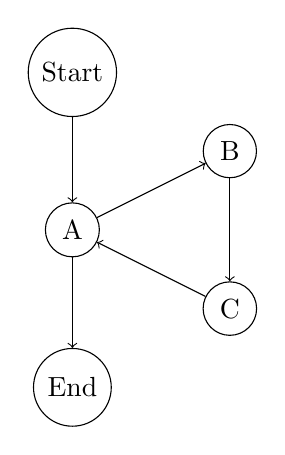
\begin{tikzpicture}
    \node[circle, draw] (start) at (4,4) {Start};
    \node[circle, draw] (a) at (4,2) {A};
    \node[circle, draw] (b) at (6,3) {B};
    \node[circle, draw] (c) at (6,1) {C};
    \node[circle, draw] (d) at (4,0) {End};


    \draw[->] (start) to node[above] { } (a);
    \draw[->] (a) to node[above] { } (b);
    \draw[->] (b) to node[above] { } (c);
    \draw[->] (a) to node[above] { } (d);
    \draw[->] (c) to node[above] { } (a);
\end{tikzpicture}

Sind dies alle Prime-Paths: \\

$ Start \rightarrow  A \rightarrow  End$ \\
$ Start \rightarrow A \rightarrow B \rightarrow C$ \\
$ A \rightarrow B \rightarrow C \rightarrow A $ \\
$ B \rightarrow C \rightarrow A \rightarrow B $ \\
$ C \rightarrow A \rightarrow B \rightarrow C $ \\
$ B \rightarrow C \rightarrow A \rightarrow End $ \\

und schon zwei Testpfade würden ausreichen um die Prime-Path Coverage zu erfüllen.
Die Testpfade die das Testrequirement erfüllen sind:

$Start \rightarrow A \rightarrow End$ \\
$Start \rightarrow A \rightarrow B \rightarrow C \rightarrow A \rightarrow B \rightarrow C \rightarrow A \rightarrow End$

\subsection{Complete-Path Coverage}

Als letztes Coveragekriterium wollen wir die Complete-Path Coverage einführen.
Ziel dieses Coveragekriteriums ist es, dass jeder mögliche Pfad mit einem Test abgedeckt werden kann.
Wir brauchen dieses Kriterium nicht ausführlich definieren, da in zyklischen Graphen eine Complete-Coverage nicht möglich ist.
Kreise in Graphen führen zu einer unendlich großen Menge an Pfaden und wir können keine unendlich große Menge behandeln.
Die Complete-Path Coverage ist sinnvoll wenn wir Kreise verbieten und der Testgraph nicht zu groß ist.
Um unsere Methode jedoch von \cite[Property-based Testing]{property-based-testing} abzugrenzen wollen wir explizit Kreise erlauben.
Ja sogar fördern um zu symbolisieren warum unsere Methode eine Verbesserung darstellt.

\subsection{abschließender Vergleich der Coverage-Kriterien}

Wir haben nun verschiedene Coverage-Kriterien kennengelernt und teilweise schon Probleme benannt die einzelne
Kriterien haben.
Im Sinne einer zufriedenstellenden Testung eines Systems wollen wir nun die einzelnen Kriterien noch einmal
zentral gegenüber stellen und sehen, welche Kriterien sich eignen würden für unseren, zu entwickelnden Prototypen.
Unser Vergleich wird 4 verschiedene Kriterien beachten, diese sind Granularität, Redundanz, Abdeckungspotential und Komplexität beziehungsweise Effizienz.
Obwohl alle Überdeckungskriterien einen einzigartigen Blick auf den Graphen bieten, so lässt sich feststellen, dass
einige Überdeckungskriterien geeigneter sind als andere.

\begin{description}
    \item[Granularität] Dieses Kriterium setzt seinen Fokus darauf, welche Teile des Graphens im Überdeckungskriterium Anwendung finden.
    Hierbei schauen wir insbesondere darauf, wie die Struktur des Graphens überdeckt wird.

    \item[Redundanz] Damit wir nicht immer wieder die selben Tests ausführen vergleichen wir, wie stark die Redundanz innerhalb
    des Überdeckungskriteriums ist. Wir wollen möglichst effizient testen da der Testprozess bei großen Systemen
    durchaus einige Zeit in Anspruch nehmen kann.
    \item[Abdeckungspotential] Wir untersuchen hier, wie stark das Potential des Kriteriums ist Tests zu generieren, die verlässlich Fehler finden.
    Hierbei ist vor allem wichtig, wie die Pfade strukturell aufgebaut sein werden die das Überdeckungskriterium erfüllen.

    \item[Komplexität / Effizienz] Mit der Komplexität und Effizienz wird untersucht, wie viele Pfade generiert werden und wie gut der mögliche Testraum durch diese
    abgebildet werden kann.
\end{description}

\newcolumntype{C}{>{\Centering\arraybackslash}X}
\begin{center}
    \begin{table}[!ht]
        \begin{tabularx}{\textwidth}{|c|c|c|c|c|}
            \hline
            \textbf{Kriterium} & \textbf{Granularität} & \textbf{Redundanz} & \textbf{Abdeckungstiefe} & \textbf{Komplexität, Effizienz}\\
            \hline
            \textbf{Node} & Knoten & Keine & Oberflächlich & Niedrigste, schnellste\\
            \hline
            \textbf{Edge} & Kanten & Minimal & Ein bisschen tiefer & Mittlere, effizient\\
            \hline
            \textbf{Edge-Pair} & Kantenpaare & Überlappung & Tiefer & Erhöhte, effizient\\
            \hline
            \textbf{SimplePath} & Pfade ohne Wiederholungen & Keine & Ziemlich tief & Hohe, langsam\\
            \hline
            \textbf{PrimePath} & Hauptpfade & Kann enthalten & Tief & Sehr hoch, langsam\\
            \hline
            \textbf{CompletePath} & Alle möglichen Pfade & Höchste & Am tiefsten & Extrem hoch, sehr langsam\\
            \hline
        \end{tabularx}
        \caption{Vergleich der Graphabdeckungskriterien}
    \end{table}
\end{center}

\section{Graphcoverage für Code}

Im Kontext der Testentwicklung erlaubt die Graphcoverage es uns, einen systematischen Ansatz zur Testgenerierung zu verfolgen.
Beziehen wir die Graphcoverage auf die Generierung von Tests für Code so müssen wir uns zuerst fragen, wie wir Code
als Graphen darstellen können.
Da dieser Abschnitt eher der generellen Einordnung dient, werden wir uns an dieser Stelle kurz halten.
Im Allgemeinen muss der Code zuerst in einen Kontrollflussgraphen überführt werden. (Quelle)
Ein Kontrollflussgraph ist ein gerichteter Graph mit, wie in 4.1 auch definiert, einer Menge Knoten, Anfangskonten und Endknoten sowie Kanten.
Wer mehr über die Umwandlung von Code in Kontrollflussgraphen lernen will, sei an \cite[Kapitel 2.]{software-testing} verwiesen.


\begin{minipage}{.5\linewidth}
    \begin{lstlisting}
function example(x, y) {
    if (x > 10) {
        if(x > 100){
            return x;
        }
        example(x - 5, y);
    } else {
        if (y < 5) {
            return y;
        }
        return x;
    }
}
    \end{lstlisting}

\end{minipage}%
\begin{minipage}{.5\linewidth}
    \begin{center}
        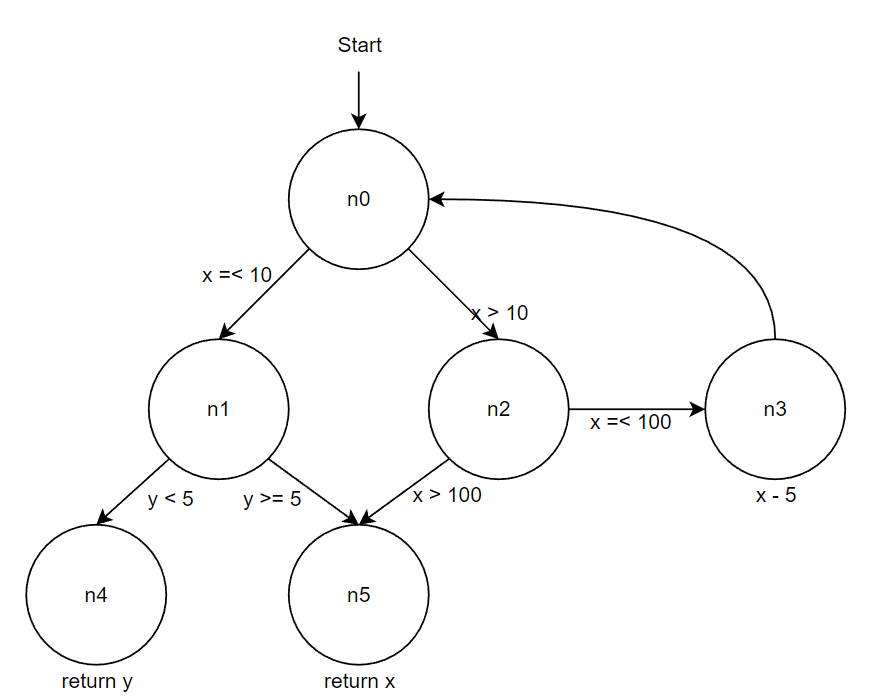
\includegraphics[width=\textwidth,height=\textheight,keepaspectratio]{img/cfg}
    \end{center}
\end{minipage}

Der Code der Funktion $example$ sei nun zu testen.
Mithilfe der zuvor definierten Coveragekriterien können wir Pfade nun Pfade ermitteln und aus diesen Pfaden tests generieren.
Nehme wir zum Beispiel die Node-Coverage.
So müssen wir Pfade finden, sodass jeder Knoten mindestens einmal in einem Test vorkommt.
Mit NodeCoverage sind die Pfade $(N_0, N_2, N_3, N_1, N_5)$ und $(N_0, N_1, N_4)$ ausreichend.
Jeder Knoten wird durch einen Pfad repräsentiert.
Erreicht werden können diese Pfade durch die Variablenauswahl x = 15, y = 10 für Pfad 1 und x = 5, y = 10 für Pfad 2.
Somit haben wir die Tests example(15,10) und example(5,10) welche NodeCoverage erfüllen.
Wir sehen auf anhieb, dass die Node-Coverage nicht ausreichend ist um Code gut zu testen.
Es ist wünschenswert, dass jede Zeile Code im Testprozess mindestens einmal ausgeführt wird (Quelle TODO).
Wir sehen aber, dass z.B. Zeile 4 nie ausgeführt wird durch unsere Tests.
Da die Tests jedoch die Node-Coverage erfüllen müssen wir schlussfolgern, dass die Node-Coverage nicht ausreichend ist.
Somit muss ein stärkeres Coverage-Kriterium her um Code ideal zu testen.
Der interessierte Leser sei an dieser Stelle an \textit{Introduction to Software Testing Kapitel 2.3.1} \cite{software-testing} verwiesen.
Wir wollten hier lediglich zeigen, dass Überdeckungskriterien speziell für den Anwendungsfall auszuwählen sind.

\section{Graphcoverage für GraphQL}

Wie wir zuvor, in $3.3$ feststellen konnten, lässt sich GraphQL in einen Graphen übersetzen.
Aus dieser Tatsache folgt, dass wir Coveragekriterien auf diesem Graphen nutzen können.
Im Unterschied zum Code ist die Zugrundeliegende Struktur direkt ein Graph und wir müssen keine großen Umwandlungen vornehmen.
Alle Informationen über den Graphen sind in seinem Schema kodiert.
Die zu ermittelnden Pfade ergeben damit auch direkt unsere Tests.
Im folgenden wollen wir untersuchen, welches Coveragekriterium denn am geeignetsten wäre um es
für Testgenerierung zu nutzen.
Wir betrachten zuerst jedes Coveragekriterium für sich, betrachten seine Fähigkeiten aber auch Limitierungen.
Abschließend ziehen wir ein Fazit, welches Coveragekriterium sich in unserem Kontext am ehesten eignen würde für
eine Testgenerierung.
Wir starten vom grobgranularsten Kriterium und verfeinern die Granularität immer weiter.

\subsection{Node-Coverage für GraphQL}

Die Node-Coverage zielt darauf ab, dass jeder Knoten in mindestens einem Test Berücksichtigung findet.
In GraphQL sind Knoten als Type definiert.
Jeder Type definiert seine eigenen Resolver wobei dies im Endeffekt Funktionen sind die es zu Testen gilt.
Nutzen wir nun Node-Coverage, so ignorieren wir unsere Maxime, dass wir möglichst alle Funktionen wenigstens einmal aufrufen wollen.
So kann ein Type mehrere Felder definieren, ist dieser Type aber in einem Pfad nur einmal mit einer Funktion vertreten, so gilt er als ausreichend abgedeckt.
Dadurch, dass die Kanten also eben so wichtig sind, ist Node-Coverage ein ungeeignetes Coveragekriterium für GraphQL Testgenerierung.

\subsection{Edge-Coverage für GraphQL}

Zuvor wurde deutlich, dass die Abdeckung aller Kanten essentiell ist um GraphQL gut zu testen.
Mit der Edge-Coverage zielen wir genau darauf ab, dass jede Kante mit mindestens einem Test abgedeckt wird.
Im Sinne unserer Maxime, dass jede Funktion zumindest einmal ausgeführt werden sollte, haben wir hier ein geeigneteres
Kriterium gefunden.
Die Edge-Coverage findet auch Anwendung in \textit{Propert-based Testing}\cite[vgl. D-RQ1 ]{property-based-testing}
Hierbei muss gesagt werden, dass Edge-Coverage durchaus unseren Zweck erfüllt, dass jede Funktion einmal ausgeführt wird.
Jedoch bezieht unser Kontext sich insbesondere auf das Integrationstesten.
Wir wollen sicherstellen, dass die Funktionen miteinander ideal funktionieren.
So ergibt sich, dass Edge-Coverage eine nicht zufriedenstellende Komplexität liefert da nur beachtet wird, dass alle Kanten einmal getest werden.
Es wird nicht beachtet, dass auch die Hintereinanderreihung der Kanten funktionieren muss, da in GraphQL eine Funktion tiefer in der Query immer auf die
Ergebnisse einer Funktion höher in der Query zurückgreift.
Um zu validieren, dass diese Zusammenarbeit klappt, brauchen wir noch speziellere Überdeckungskriterien.

\subsection{Edge-Pair-Coverage für GraphQL}

In der Edge-Pair Coverage betrachten wir alle Kantenpaare.
Dadurch erlangen wir eine bessere Abdeckung der Funktionen indem sichergestellt wird, dass jede Kante mit jeder darauffolgenden Kante einmal ausgeführt wird.
Dieses Kriterium stellt eine Verbesserung der Edge-Coverage dar, allerdings werden eben nur aufeinanderfolgende Kantenpaare abgedeckt.
GraphQL kann aber wesentliche tiefere und komplexere Strukturen abbilden.
Somit ergibt sich, dass die Abdeckung mit Edge-Pair noch nicht ausreichend ist da insbesondere stark verschachtelte Anfragen
hier nicht als Test generiert werden obwohl diese wahrscheinlich besonders interessant für Tests sind.

\subsection{SimplePath-Coverage für GraphQL}

SimplePath berücksichtigt alle Pfadkombinationen im Schema die keine Wiederholungen enthalten.
Mit diesem Coveragekriterium haben wir ein Kriterium gefunden, dass zumindest die einfachen Pfade, ohne Kreise gut abdeckt.
Wir können theoretisch also folgern, dass dieses Kriterium gut geeignet wäre.
Praktisch angewandt zeigt sich jedoch schnell, dass dieses Kriterium sehr viele redundante Tests erzeugt.
Was per-se nicht schlecht ist jedoch keinen großen Informationsgewinn bringt.

\subsection{Prime-Path Coverage für GraphQL}

Mit der PrimePath Coverage elimieren wir die Redundanz aus der SimplePath Coverage und stellen sicher, dass
vor allem sehr relevante Pfade gefunden werden die wir zur Testabdeckung nutzen.
Wir erhöhen so die Effizienz der Tests indem wir unrelevante Tests filtern und dennoch eine zufriedenstellende Abdeckung beibehalten.

\subsection{Complete-Path Coverage für GraphQL}

Mit der Complete-Path Coverage haben wir als Ziel, dass wir alle Pfade, die möglich sind, auch generieren und in unseren
Tests berücksichtigen.
Da GraphQL jedoch Zyklen erlaubt ist die Anzahl an potentiellen Pfaden unendlich.
Hierdurch folgt, dass auch der Testraum unendlich werden würde mit der Complete-Path Coverage.
Somit ist Complete-Path Coverage nicht umsetztbar da wir im Allgemeinen nicht ausschließen können und wollen, dass GraphQL
keine Zyklen haben kann.
Dies wäre ein zu großer Einschnitt in GraphQL die von einem Testtool nicht erwartet werden sollte.

\subsection{Fazit}

Die beiden geeignetsten Coveragekriterien sind SimplePath-Coverage und PrimePath Coverage wobei PrimePath Coverage hierbei
als Verfeinerung bzw. Einschränkung von SimplePath gesehen werden kann.
Da jeder PrimePath auch ein SimplePath ist.
Es hängt nun vom SUT ab welches Kriterium zu nutzen ist.
Im Allgemeinen lässt sich sagen, dass wir SimplePath-Coverage nutzen sollten für kleinere, einfachere Schemas da
wir somit eine gute Testabdeckung erreichen und die Offside der großen Redundanz noch nicht so schnell zu tragen kommt.
Sollte das Schema nun stark wachsen und insbesondere viele Zyklen aufweisen, so empfiehlt sich die PrimePath Coverage da
sie viel Redundanz entfernt.
